\section{Introduction}

The domain of stream programs is important because it stands at the
intersection of trends in applications and architectures.  Stream
programming naturally represents applications such as audio, video,
digital signal processing, and data analysis; applications that are
increasingly prevalent as computing moves towards data-centric
applications and to the mobile and embedded space.  Also, by virtue of
their structure -- a graph of independent computational nodes (termed
{\it filters}) with explicit and regular communication -- stream
programs are a natural fit for exploiting coarse-grained parallelism
suitable for multicore architectures.  The interest in streaming
applications has spawned a number of streaming languages that target
the streaming domain, including StreamIt~\cite{streamitcc},
Brook~\cite{brook04}, Cg~\cite{cg03},
SPUR~\cite{spur05samos}, Spidle~\cite{spidle03}, Lime~\cite{lime10},
and SPL~\cite{spl09}.

The key to effectively parallelizing stream programs is to take
advantage of data parallelism present in filters that do not maintain
state~\cite{gordon-asplos06}.  Data parallelism provides load-balanced
and limitless parallelism (as long as input data is
available). However, many real-world streaming applications include
filters with explicit {\it induction variable} state. This is state
that is derived from the number of executions of the filter. For
example, a filter may keep track of how many times it has been
invoked, in order to perform a special action every N iterations. An
MPEG encoder has a concrete example of such a filter; running counters
are used to maintain positions in a two-dimensional array.  The
presence of induction variable state inhibits data parallelism, and
represents a bottleneck for parallelization scalability of the
application.

\begin{figure}[t!]
\centering
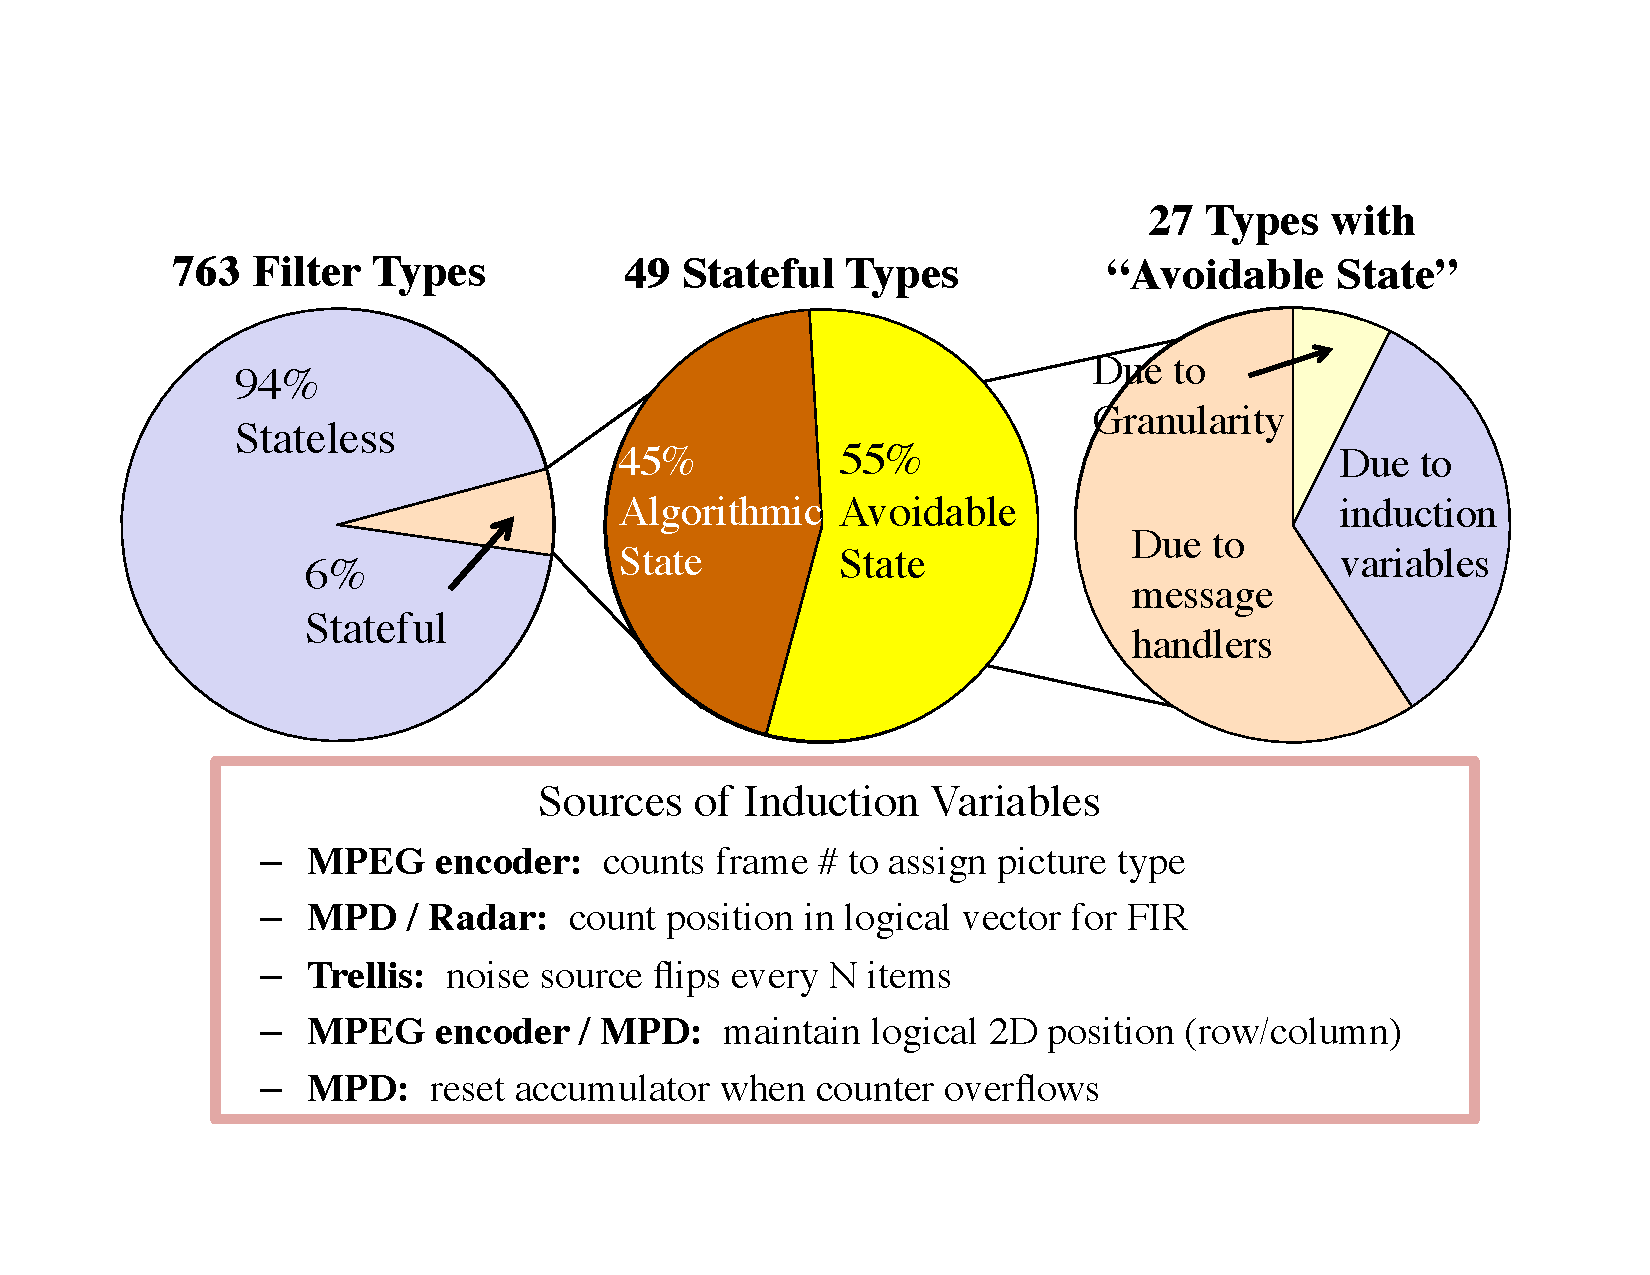
\includegraphics[width=3.4in]{figures/state-figure.pdf}
\caption{A summary of the findings of~\cite{streamit-suite}.  Of the
  763 filters of 65 programs (over 35k lines of code), 55\% of
  stateful filters include avoidable state, and much of that is due to
  induction variable state in real world
  applications.\protect\label{fig:state}}
\end{figure}

 
In this paper we introduce techniques to represent, capture, and
parallelize induction variable state in stream programs. Our research
is conducted in the context of the StreamIt programming
language~\cite{streamitcc}.  Figure~\ref{fig:state} summarizes the
finding of~\cite{streamit-suite} in regards to induction variable
state on the StreamIt benchmark suite.  Of the 65 benchmarks included
in the suite many of the real world applications include induction
variable state, including MPEG encoder, beamforming, Trellis, and MPD.
It is important to represent induction variable state because it is a
common implementation idiom and parallelizing such state removes
scalability bottlenecks to drastically improve parallelization
performance. As we will show, even a small amount of stateful
computation will severely limit parallelization scalability as we
quickly transition to the manycore era with hundreds and thousands of
cores.

We represent induction variable state by introducing a new expression
keyword to the StreamIt language. The new expression, {\tt iter()},
when executed, evaluates to the current execution number of a filter.
Induction variable state and control flow can be represented as simple
expressions that include the {\tt iter()} expression, precluding the
need for the programmer to explicitly maintain induction state. We
provide a simple desugaring that converts a filter that employs the
{\tt iter()} expression into a filter maintains explicit induction
variable state.

Automatic induction variable recognition algorithms are inadequate
because their idiomatic nature could not capture all the real-world
cases of induction variable state in the benchmarks.  Furthermore, we
found that the {\tt iter()} keyword simplified implementation of
filters that included induction variable calculation or control flow.
Programmers are enticed to utilize the keyword because it naturally
captures a common implementation pattern.

We extend the StreamIt compiler to be fully aware of the new keyword.
Most importantly, we modify StreamIt's source-to-source filter 
data-parallelization transformation, termed {\it
  fission}~\cite{streamit-asplos}, to correctly parallelize filters
that utilize the new keyword. Our formulation correctly calculates the
iteration number across data parallel duplicates of the original
filter, taking into account the fact that the iterations of the original
filter are now split across the duplicates. Furthermore, we show how
the modified fission transformation must interact with the
steady-state scheduling algorithm of the
compiler~\cite{karczmarek-lctes03} since it may modify the
distribution of iterations between the parallelization duplicates.

The necessity of representing induction variable state and the
effectiveness of our parallelization technique is demonstrated via a
case study of the StreamIt implementation of the motion estimation
stage of MPEG2 encoding~\cite{ipdps2006}. The motion estimation stage
is the most computationally intensive stage of encoding, accounting
for at least a third of the total computation in the entire MPEG2
encoder~\cite{drake-thesis}. A static estimation calculates that 98\%
of the work of the stage is concentrated in filters that include
induction variable state. Originally, these filters cannot be data
parallelized because of the presence of state. After modification of
these filters to utilize the {\tt iter()} keyword, the entire
application is data parallel. The StreamIt compiler, employing our
modified fission transformation is able to get significant speedups
for the modified version (use of {\tt iter()}) over the unmodified
version (with explicit induction state) targeting a commodity
multicore SMP processor: 5X for 8 cores, 9X for 16 cores, and 16X for
32 cores.

This work expands the domain of algorithms for which the stream
programming model, and its associated compiler technologies, is
effective at automatically managing parallelism. For automatic
parallelization to become mainstream, computer scientists must
continue to remove common sensitivities (in this case induction
variable state) that inhibit parallelization.

This paper makes the following contributions:

\mybegin

\myitem{Directly represent the basis of induction variable state in
  the language}. We introduce a new expression that is attractive to
  programmers and precludes the need for a programmer to maintain
  induction state in a stream program.

  \myitem{Automatic parallelization of induction variable state}. We
  provide modifications to the foundational parallelization
  transformation of the StreamIt language so that it can
  data parallelize filters with induction variable state utilizing the
  {\tt iter()} expression.

\myitem{Case study of induction variable state}. We include a
motivating case study of applications from the StreamIt benchmark
suite that include induction variable state.  Furthermore, we
demonstrate the benefits of our approach via the motion estimation
stage of MPEG2 encoding.

\myend

The remainder of this paper is organized as follows:
\S\ref{sec:streamit} introduces the StreamIt language, \todo{finish}.

% ----

% With a growing need to scale programs more effectively with multicore 
% architectures, programs need to be written such that they efficiently exploit 
% parallelism across many cores.  Stream programs offer an attractive approach to 
% exposing such parallelism.  Furthermore, this domain is well-suited over many 
% applications including audio, video, and digital signal processing.  

% The stream programming paradigm exposes much parallelism by virtue of the 
% structure of the programs written.  Stream programs are constructed as a set of 
% independently processing actors that communicate via data channels.  These 
% actors are fired repeatedly on a periodic schedule.  Dependencies between 
% actors are derived largely through communication channels.  Accordingly, 
% compilers can very easily introduce parallel execution by leveraging this 
% dependence information and the independent nature of the actors.

% The parallelism exposed in stream programs can be classified in a variety of different ways.  The stream graph, representing how the actors of the corresponding stream program communicate with one another, can be partitioned in many ways and assigned to cores accordingly.  It is important to partition the graph in such a way that you leverage the right combination of task, data, and pipeline parallelism.

% Task parallelism refers to a pair of actors that operate on different parallel branches such that outputs to one will never reach the input of the other.  This form of parallelism is simple to exploit, as each actor can be assigned to independent cores.

% Pipeline parallelism refers to chains of actors that are directly connected in the stream graph.  Accordingly, the producer and consumer of data in each chain can be assigned to independent cores.  Communication between actors can be maintained using an on-chip network.

% Data parallelism refers to stateless actors.  Such actors have no dependencies between execution steps.  Because the execution of these actors are independent, it is possible to assign different execution steps to independent cores.  In exposing this form of parallelism, the stateless actor would be replicated and assigned to various cores so that multiple parts of the input stream can be manipulated in parallel.

% Data parallelism can be inhibited when presented with actors that must maintain mutable state between execution steps.  Such actors cannot be replicated and executed independently and in parallel because each of these execution steps are dependent on previous execution steps.  While this may not inhibit task or pipeline parallelism, this does obscure potential data parallelism opportunities.

% A common category of state that actors maintain is that of induction state.  Several actors are written so that execution is dependent on the number of times the actor is executed.  Common usage of induction state includes ..... [thies pact10]

% In this paper, we propose eliminating induction variable from actor state by providing a new language construct.  This construct provides the current iteration value of the corresponding actor, indicating how many times this actor has been invoked.  This construct introduces internal state to the actor that acts as an iteration counter.  The compiler is able to leverage built-in capabilities to expose data parallelism in actors on filters that maintain this internal state.\cite{mgordon-phd}   


